\chapter{Sistema para Controle de Clientes}\label{cap:sistemaControleClientes}
\epigraph{``\textit{É fazendo que se aprende a fazer aquilo que se deve aprender a fazer}''.}{Aristóteles}

\lettrine[lines=4, lhang=0.1, lraise=0, loversize=0.2, findent=0.1em]{\textcolor{corTema}{N}}{ESTE} Capítulo teremos como objetivos entender e realizar a construção de uma aplicação Web em Java completa.


\section{Introdução}

Chegou a hora de colocar em prática tudo o que aprendemos nos Capítulos anteriores com o objetivo de criar uma aplicação Web em Java completa. Iremos passar por todos os passos do desenvolvimento da aplicação para que no Capítulo~\ref{cap:primeiroProjeto}, você possa usar um conjunto de requisitos para desenvolver um sistema sozinho. Vamos começar?


\section{Analisando os Requisitos}

Imagine que fomos contratados para criar um sistema para controle de cadastro de clientes. Esse sistema deve manter vários dados de um cliente: nome, sobrenome, data de nascimento, CPF, e-mail, logradouro, número, bairro, cidade e CEP. O contratante também deseja que seja possível manter um cadastro de cidades e de estados, sendo que as cidades devem ter um nome e um estado, enquanto um estado deve ter um nome e uma sigla. Cada um dos cadastros (cliente, cidade e estado), deve conter as funcionalidades de inserir, alterar e excluir um determinado registro.

Vamos analisar esses requisitos. Primeiramente, vamos identificar os tipos de entidades que farão parte do sistema, fazendo a seguinte pergunta: Quais são os tipos de ``coisas'' que o sistema deve gerenciar? O sistema deve manter um cadastro de Clientes, um cadastro de Cidades e um cadastro de Estados. Sendo assim, identificamos três entidades, ou seja, Cliente, Cidade e Estado.

Cada um desses tipos de entidade tem uma determinada lista de características ou atributos. Vamos organizá-las em uma tabela. Veja essa organização na Tabela~\ref{tab:caracteristicasEntidades}.

\FloatBarrier
\begin{table}[ht]
    \centering
    \caption{Atributos dos tipos de entidade}
	\begin{tabular}{cl}
	    \hline
	        \textbf{Entidade}     & \textbf{Atributos (características)} \\ \hline
	    \multirow{10}{*}{Cliente} & - nome                                 \\
	                              & - sobrenome                            \\
	                              & - data de nascimento                   \\
	                              & - CPF                                  \\
	                              & - e-mail                               \\
	                              & - logradouro                           \\ 
	                              & - número                               \\
	                              & - bairro                               \\
	                              & - Cidade                               \\
	                              & - CEP                                  \\ \hline
	     \multirow{2}{*}{Cidade}  & - nome                                 \\
	                              & - Estado                               \\ \hline
	     \multirow{2}{*}{Estado}  & - nome                                 \\
	                              & - sigla                                \\ \hline
	\end{tabular}
    \\ \vspace{0.2cm}
    \textbf{Fonte:} Elaborada pelo autor
    \label{tab:caracteristicasEntidades}
\end{table}
\FloatBarrier

Sabemos que esses tipos de entidade que foram identificados se tornarão tabelas na nossa base de dados relacional não é mesmo? Cada atributo de cada tipo de entidade se tornará uma coluna na tabela correspondente. Sabemos também que cada registro de uma determinada tabela precisa ser diferenciado dos outros não é mesmo? Para isso analisamos as tabelas até que consigamos identificar as chaves primárias de cada uma delas. Uma chave primária é o conjunto mínimo de um ou mais atributos de um determinado tipo de entidade que garante a unicidade de um registro, sendo assim, precisamos encontrar, na lista de características de cada entidade, uma ou mais características que, usadas em conjunto, garantem que um registro é diferente de outro. Tomemos como exemplo o tipo de entidade Estado. Veja na Tabela~\ref{tab:exemplosEstados} uma lista de registros da tabela \texttt{estado} do nosso provável banco de dados.

\FloatBarrier
\begin{table}[ht]
    \centering
    \caption{Exemplos de registros da tabela ``estado''}
	\begin{tabular}{cc}
	    \hline
	    \multicolumn{2}{l}{\textbf{Tabela: estado}} \\ \hline
	    \textbf{nome}  &       \textbf{sigla}       \\ \hline
	      São Paulo    &             SP             \\ \hline
	    Rio de Janeiro &             RJ             \\ \hline
	     Minas Gerais  &             MG             \\ \hline
	         ...       &            ...             \\ \hline
	\end{tabular}
    \\ \vspace{0.2cm}
    \textbf{Fonte:} Elaborada pelo autor
    \label{tab:exemplosEstados}
\end{table}
\FloatBarrier

O que diferencia um estado de outro? Se usarmos os atributos \texttt{nome} e \texttt{sigla}, nós sempre teremos um estado diferente do outro, ou seja, não seria permitido a criação de um novo estado que tivesse o mesmo nome \textbf{e} a mesma sigla do que ume estado que já existe na tabela, concorda? Agora pense, e se usarmos apenas o \texttt{nome} ou somente a \texttt{sigla}, qual seria suficiente? Temos então três opções para definir a chave primária dessa tabela. Podemos usar \texttt{nome} \textbf{e} \texttt{sigla}, somente \texttt{nome} ou somente \texttt{sigla}. Dentre essas três opções, qual ou quais são as que têm o menor conjunto de atributos? Somente \texttt{nome} ou somente \texttt{sigla}, correto? Como temos duas opções, podemos escolher qualquer uma delas, desde que, para o cenário ou ``minimundo'' que está sendo modelado, um desses atributos garanta a unicidade de tupla. Vamos dizer que nós escolhemos a opção de definir a chave primária da tabela usando o atributo \texttt{sigla}. Legal, agora sabemos que um Estado é diferenciado do outro pela sua sigla, então não pode existir mais de um registro com a mesma sigla.

Agora temos outro problema: o desempenho do banco de dados. Quando criarmos a tabela \texttt{cidade}, esta vai ter que referenciar a tabela \texttt{estado}, usando uma coluna que vai ter o mesmo tipo da coluna que representa a chave primária da tabela \texttt{estado}. Essa coluna, como você deve se lembrar, é denominada chave estrangeira. Como cada estado tem uma sigla de dois caracteres, sempre que um estado for referenciado em um registro da tabela \texttt{cidade}, essa referência vai ter que ter o mesmo valor do registro contido na tabela sigla. Apesar de essa abordagem funcionar, nós podemos atacar esse problema de outra forma. Podemos definir que a coluna \texttt{sigla} tem valor único (\textit{unique}) nos registros da tabela \texttt{estado} e então criar uma chave primária que contém apenas um número. Essa chave primária é chamada de chave artificial, ou \textit{surrogate}, sendo que normalmente é chamada de \texttt{id} (identificador). Note que como o próprio nome diz, essa chave é artificial. O que vai garantir a unicidade dos registros é a configuração de cada uma das colunas.

O que ganhamos com isso? Ganhamos desempenho, pois estamos usando números para referenciar colunas de outras tabelas, não Strings. Imagine definir a chave primária de um Cliente como CPF. Ao precisarmos referenciar um cliente em outra tabela, digamos uma tabela de \texttt{pedidos}, precisaríamos ter uma cópia do CPF do cliente em cada pedido, gastando cerca de 11 a 14 caracteres (um CPF é no formato 000.000.000-00), ao passo que poderíamos usar apenas um número! Veja, se cada caractere ocupar 4 bytes em disco/memória, um CPF de 11 dígitos (só os números) ocupará 44 bytes (352 bits), enquanto um número inteiro provavelmente ocupará 4 ou 8 bytes (32 ou 64 bits). Pense nas implicações! Sabendo de tudo isso, podemos partir para o projeto do banco de dados.


\section{Projetando Banco de Dados}

Não irei documentar aqui todo o processo de projeto do banco de dados, que vai desde a análise dos requisitos, passando pela criação do DER (Diagrama Entidade-Relacionamento) até a implementação do modelo físico, pois este não é o objetivo deste livro, mas note que no desenvolvimento de um sistema esses passos são normalmente realizados. Iremos partir diretamente para a implementação do modelo físico. Antes de criarmos o código escrito em \textit{Structured Query Language} (SQL) para a criação da estrutura da nossa base de dados, vamos organizar os atributos das nossas tabelas –que são baseadas nas características dos tipos de entidade– e especificar suas características. Veja a Tabela~\ref{tab:detalhesTabelas}.

\FloatBarrier
\begin{table}[ht]
    \centering
    \caption{Detalhamento das colunas de cada tabela}
	\begin{tabular}{cllc}
	    \hline
	         \textbf{Tabela}      & \textbf{Coluna}                         & \textbf{Tipo}               & \textbf{É único?} \\ \hline
	    \multirow{11}{*}{cliente} & \texttt{id\textsuperscript{*}}          & \inlineSQLCode{INT}         &         x         \\
	                              & \texttt{nome}                           & \inlineSQLCode{VARCHAR(45)} &                   \\
	                              & \texttt{sobrenome}                      & \inlineSQLCode{VARCHAR(45)} &                   \\
	                              & \texttt{dataNascimento}                 & \inlineSQLCode{DATE}        &                   \\
	                              & \texttt{cpf}                            & \inlineSQLCode{VARCHAR(14)} &         x         \\
	                              & \texttt{email}                          & \inlineSQLCode{VARCHAR(60)} &                   \\
	                              & \texttt{logradouro}                     & \inlineSQLCode{VARCHAR(50)} &                   \\
	                              & \texttt{numero}                         & \inlineSQLCode{VARCHAR(6)}  &                   \\
	                              & \texttt{bairro}                         & \inlineSQLCode{VARCHAR(30)} &                   \\
	                              & \texttt{cep}                            & \inlineSQLCode{VARCHAR(9}   &                   \\
	                              & \texttt{cidade\_id\textsuperscript{**}} & \inlineSQLCode{INT}         &                   \\ \hline
	     \multirow{3}{*}{cidade}  & \texttt{id\textsuperscript{*}}          & \inlineSQLCode{INT}         &         x         \\
	                              & \texttt{nome}                           & \inlineSQLCode{VARCHAR(30)} &                   \\
	                              & \texttt{estado\_id\textsuperscript{**}} & \inlineSQLCode{INT}         &                   \\ \hline
	     \multirow{3}{*}{estado}  & \texttt{id\textsuperscript{*}}          & \inlineSQLCode{INT}         &         x         \\
	                              & \texttt{nome}                           & \inlineSQLCode{VARCHAR(30)} &                   \\
	                              & \texttt{sigla}                          & \inlineSQLCode{VARCHAR(2)}  &         x         \\ \hline
	    \multicolumn{4}{l}{\textsuperscript{\texttt{ *}} chave primária}                                                      \\ \hline
	    \multicolumn{4}{l}{\textsuperscript{\texttt{**}} chave estrangeira}                                                   \\ \hline
        \multicolumn{4}{l}{todas as colunas são não nulas (\texttt{NOT NULL})}                                                \\ \hline
	\end{tabular}
    \\ \vspace{0.2cm}
    \textbf{Fonte:} Elaborada pelo autor
    \label{tab:detalhesTabelas}
\end{table}
\FloatBarrier

Usei o MySQL Workbench para criar um diagrama do nosso modelo físico. Veja como ficou na Figura~\ref{fig:cap05ModeloFisico}.

\FloatBarrier
\begin{figure}[!htbp]
    \centering
    \caption{Diagrama do modelo físico da base de dados}
    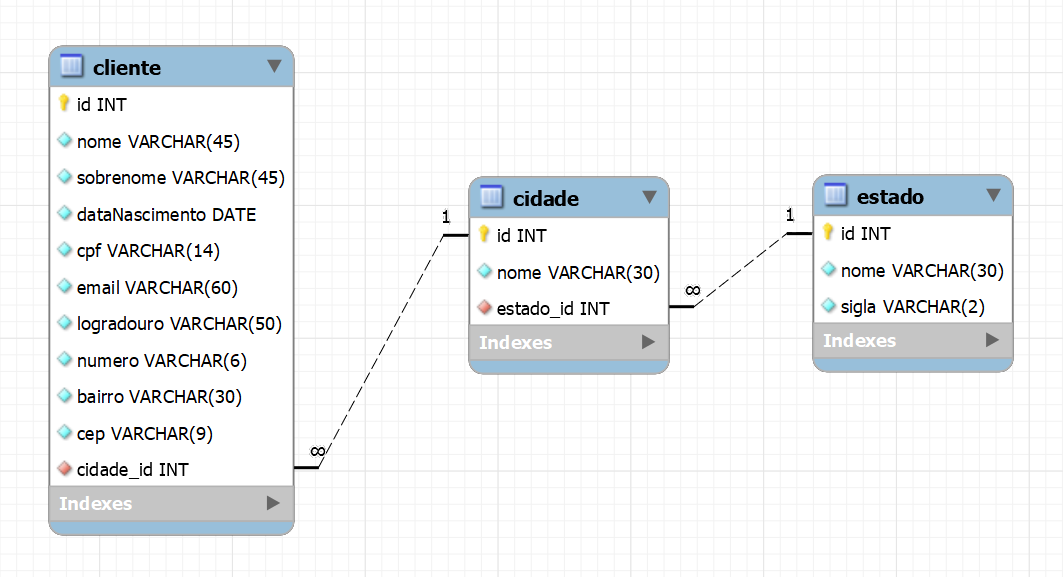
\includegraphics[scale=0.5]{imagens/cap05ModeloFisico}
    \\\textbf{Fonte:} Elaborada pelo autor
    \label{fig:cap05ModeloFisico}
\end{figure}
\FloatBarrier

Vamos agora implementar o banco de dados. No MySQL Workbench, crie uma nova base de dados com o nome de \texttt{cadastro\_clientes} como feito na Seção~\ref{sec:preparandoAmbiente}. Com a base criada, torne-a padrão, abra uma aba para digitar código SQL e copie o código da Listagem~\thechapter.\ref{listagem:projetos/capitulo05/banco/estado.sql} no editor e execute o \textit{script}.

\sqlCode{\textit{Script} SQL para criação da tabela ``estado''}{projetos/capitulo05/banco/estado.sql}

Faça o mesmo processo para a Listagem~\thechapter.\ref{listagem:projetos/capitulo05/banco/cidade.sql} e para a Listagem~\thechapter.\ref{listagem:projetos/capitulo05/banco/cliente.sql}.

\sqlCode{Script SQL para criação da tabela ``cidade''}{projetos/capitulo05/banco/cidade.sql}

\sqlCode{Script SQL para criação da tabela ``cliente''}{projetos/capitulo05/banco/cliente.sql}

Ao fazer esses três passos, temos nossas três tabelas criadas dentro da base de dados. Expanda o banco \texttt{cadastro\_clientes} e então expanda o nó \destaque{\textit{Tables}}. Lá dentro estarão as três tabelas criadas. Muito bem, terminamos a implementação do banco. Vamos agora criar um diagrama de classes para representar cada uma das nossas entidades, que serão mapeamentos das nossas tabelas no mundo orientado a objetos.


\section{Criando o Diagrama de Classes}

Para criar nosso diagrama de classes UML eu usei a ferramenta Astah UML. Existem diversas ferramentas de modelagem gratuítas. Infelizmente o Astah não poussi mais esse tipo de versão desde 2018. Você pode usar qualquer uma caso queria fazer a modelagem, mas ela não é obrigatória. Como já disse cada tabela do nosso banco de dados vai ter uma representação na nossa aplicação. Essa representação, como você já sabe, é criada usando classes. No diagrama de classes da Figura~\ref{fig:cap05DiagramaClasses}, você pode ver as três classes que representam nossas entidades. Note que cada classe contém uma série de atributos privados, denotados pelo sinal de ``\texttt{-}'', que representam as colunas da tabela e que o acesso a esses atributos é feito usando os métodos \texttt{get} e \texttt{set} correspondentes, omitidos no diagrama.

\FloatBarrier
\begin{figure}[!htbp]
    \centering
    \caption{Diagrama de classes das entidades}
    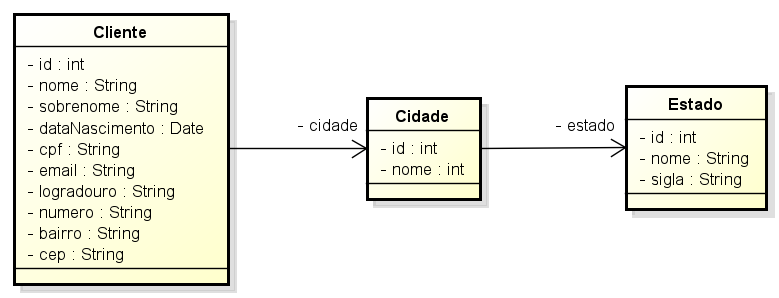
\includegraphics[scale=0.6]{imagens/cap05DiagramaClasses}
    \\\textbf{Fonte:} Elaborada pelo autor
    \label{fig:cap05DiagramaClasses}
\end{figure}
\FloatBarrier

Outro detalhe é que criei apenas o diagrama das classes que são as entidades do sistema, não me preocupando com as outras classes que nosso sistema conterá. Novamente, como no exemplo do nosso banco de dados, em um sistema de verdade, normalmente são desenvolvidos diagramas de classes muito mais completos e complexos, dependendo do nível de representação que se deseja, bem como outros tipos de diagramas UML que forem necessários. Com tudo isso pronto, podemos partir para o desenvolvimento do sistema propriamente dito! Novamente, essa não é a nossa preocupação neste livro.


\section{Construindo o Sistema}

Antes de qualquer coisa precisamos fazer um ajuste no GlassFish, pois ele precisa que todas as biblitecas/APIs que não fazem parte do Java \textit{Standard Edition} (SE), ou do Java/Jakarta EE, sejam fornecidas à ele. Para isso, faça uma cópia do arquivo \texttt{.jar} do \textit{driver} JDBC do MariaDB para o diretório:

\destaque{\texttt{C:\textbackslash Users\textbackslash <SeuUsuário>\textbackslash glassfish5\textbackslash glassfish\textbackslash domains\textbackslash domain1\textbackslash lib\textbackslash}}

Com isso, nossa aplicação poderá usar o \textit{driver} quando estiver implantada no servidor, mas note que ainda precisaremos configurá-lo do projeto, visto que ele será necessário no processo de \textit{build}.

Agora nossa tarefa será criar o projeto no NetBeans. Para isso, abra o NetBeans e crie um novo projeto do tipo Java Web com o nome de ``CadastroClientes'' (sem as aspas). Siga os passos que você tem seguido em todos os projetos criados, além de, é claro, configurar a bibliteca do \textit{driver} JDBC do MariaDB, como descrito no Capítulo~\ref{cap:padroesDeProjeto}. Em \destaque{\textit{Source Packages}}, crie o pacote ``\texttt{cadastroclientes}'' (sem as aspas) e, dentro dele, os pacotes ``controladores'', ``dao'', ``entidades'', ``jdbc'' e ``testes'' dentro do pacote ``cadastroclientes''. Em \destaque{\textit{Web Pages}}, crie os diretórios ``\texttt{css}'' e ``\texttt{formularios}'' (sem acento) e dentro deste, crie os diretórios ``\texttt{cidades}'', ``\texttt{clientes}'' e ``\texttt{estados}''. Apague o arquivo \texttt{index.html} e crie um arquivo JSP chamado \texttt{index.jsp}. Veja na Figura~\ref{fig:cap05EstruturaProjeto} como deve ficar a estrutura do projeto. Ignore os pacotes \texttt{...filtros} e \texttt{...servicos} por enquanto!

\FloatBarrier
\begin{figure}[!htbp]
    \centering
    \caption{Estrutura do projeto}
    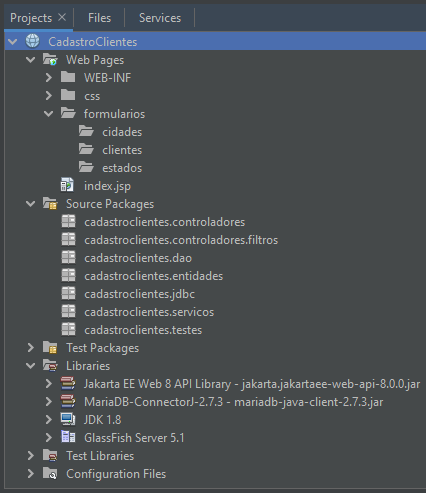
\includegraphics[scale=0.7]{imagens/cap05EstruturaProjeto}
    \\\textbf{Fonte:} Elaborada pelo autor
    \label{fig:cap05EstruturaProjeto}
\end{figure}
\FloatBarrier

Com a estrutura configurada, vamos agora copiar algumas classes do projeto ``PadroesEmPatrica'' que criamos no Capítulo~\ref{cap:padroesDeProjeto}. Para isso abra esse projeto, se ainda não estiver aberto, no NetBeans. Expanda o pacote ``\texttt{padroesempratica.jdbc}'', clique com o botão direito no arquivo ``\texttt{ConnectionFactory.java}'' e escolha \destaque{\textit{Copy}}. Volte ao projeto ``CadastroClientes'', clique com o botão direito no pacote ``cadastroclientes.jdbc'', escolha \destaque{\textit{Paste}} e então \destaque{\textit{Refactor Copy...}}. Um diálogo será aberto. Clique no botão \destaque{\textit{Refactor}}. O arquivo será copiado para o projeto e as alterações que forem necessárias fazer no arquivo, como mudar a cláusula \inlineJavaCode{package}, serão feitas pelo NetBeans. Faça o mesmo processo para o arquivo ``DAO.java'' contido no pacote ``pradoesempratica.dao'' do projeto ``PadroesEmPratica'', copiando-o no pacote ``cadastroclientes.dao'' do projeto ``CadastroClientes''. Talvez o NetBeans aponte um erro no arquivo depois da cópia. Para corrigir, abra o arquivo no editor e altere o \inlineJavaCode{import} que está com problema. 

Outro detalhe é que precisamos mudar a URL da nossa fábrica de conexões para fazer com que as conexões criadas sejam relativas à base de dados \texttt{cadastro\_clientes}. Para isso, abra o arquivo ``\texttt{ConnectionFactory.java}'' do pacote\linebreak%
``\texttt{cadastroclientes.jdbc}'' e mude a URL de:

\destaque{\texttt{jdbc:mariadb://localhost/testes\_padroes}}

Para:

\destaque{\texttt{jdbc:mariadb://localhost/cadastro\_clientes}}

Agora vamos preparar toda a camada de persistência. No pacote\linebreak%
``\texttt{cadastroclientes.entidades}'', crie três classes: ``\texttt{Estado}'', ``\texttt{Cidade}'' e ``\texttt{Cliente}'' (sem as aspas). Nas três listagens a seguir estão listados os códigos-fonte das três classes. Note que estou omitindo os gets e os sets, mas isso não significa que eles não devam existir. Fica por sua conta criá-los ok? Não se esqueça de fazer isso!

\javaCode{Entidade ``Estado''\newline%
Arquivo: \texttt{cadastroclientes/entidades/Estado.java}}{projetos/capitulo05/CadastroClientes/src/java/cadastroclientes/entidades/Estado.java}

\javaCode{Entidade ``Cidade''\newline%
Arquivo: \texttt{cadastroclientes/entidades/Cidade.java}}{projetos/capitulo05/CadastroClientes/src/java/cadastroclientes/entidades/Cidade.java}

\javaCode{Entidade ``Cliente''\newline%
Arquivo: \texttt{cadastroclientes/entidades/Cliente.java}}{projetos/capitulo05/CadastroClientes/src/java/cadastroclientes/entidades/Cliente.java}

Com as entidades prontas, vamos criar os DAOs. No pacote ``\texttt{cadastroclientes.dao}'', crie três classes: ``\texttt{EstadoDAO}'', ``\texttt{CidadeDAO}'' e ``\texttt{ClienteDAO}''. O código-fonte de cada uma dessas classes é apresentado nas listagens a seguir.

\javaCode{Código da classe ``EstadoDAO''\newline%
Arquivo: \texttt{cadastroclientes/dao/EstadoDAO.java}}{projetos/capitulo05/CadastroClientes/src/java/cadastroclientes/dao/EstadoDAO.java}

\javaCode{Código da classe ``CidadeoDAO''\newline%
Arquivo: \texttt{cadastroclientes/dao/CidadeDAO.java}}{projetos/capitulo05/CadastroClientes/src/java/cadastroclientes/dao/CidadeDAO.java}

\javaCode{Código da classe ``ClienteDAO''\newline%
Arquivo: \texttt{cadastroclientes/dao/ClienteDAO.java}}{projetos/capitulo05/CadastroClientes/src/java/cadastroclientes/dao/ClienteDAO.java}

Quantos códigos hein? Copiou tudo? Crie algumas classes de teste no pacote\linebreak%
``\texttt{cadastroclientes.teste}'' e teste a persistência de cada entidade. Com isso, terminamos a parte da persistência do nosso projeto.

Agora nós vamos começar a implementar as visualizações e os controladores. Nossa aplicação terá três \textit{links} no \texttt{index.jsp}, sendo que cada \textit{link} levará a um determinado cadastro. Cada cadastro vai conter uma página principal onde todos os itens desse cadastro serão exibidos e onde poderão ser alterados, excluídos ou então poderemos cadastrar um novo item.

Vamos começar pelo cadastro de estados. Na pasta ``\texttt{estados}'' dentro da pasta\linebreak%
``\texttt{formularios}'', crie um arquivo JSP com o nome de ``\texttt{listagem.jsp}'' (sem as aspas). Nesse arquivo vão ser listados todos os estados, portanto precisamos obter esses estados de alguma forma. Você se lembra que nos nossos DAOs existe um método chamado \inlineJavaCode{listarTodos()} que retorna todos os registros de uma determinada tabela? Nós não vamos usar esse método diretamente no JSP, então vamos criar uma classe de serviços que vai instanciar o DAO, gerar a lista e fechar a conexão para nós. Nos pacotes de código-fonte, crie um novo pacote dentro do ``\texttt{cadastroclientes}'' chamado ``\texttt{servicos}'' (sem o ``ç''). Nesse pacote, crie uma classe chamada ``\texttt{EstadoServices}'' (sem as aspas). Essa classe vai ter apenas um método, chamado \inlineJavaCode{getTodos()}, que retornará uma lista de estados. Veja o código-fonte dela na Listagem~\thechapter.\ref{listagem:projetos/capitulo05/CadastroClientes/src/java/cadastroclientes/servicos/EstadoServices.java}.

\javaCode{Código-fonte da classe de serviços para Estados\newline%
Arquivo: \texttt{cadastroclientes/servicos/EstadoServices.java}}{projetos/capitulo05/CadastroClientes/src/java/cadastroclientes/servicos/EstadoServices.java}

Criamos essa classe para que ela encapsule todo o processo de obtenção da lista de estados. Note que é no método \inlineJavaCode{getTodos()} que o \texttt{EstadoDAO} vai ser instanciado e gerenciado.

Agora que temos o JSP que vai obter a lista de estados para nós, além de gerenciar o DAO, nós podemos implementar o nosso arquivo de listagem de estados. Abra o arquivo \texttt{/formularios/estados/listagem.jsp} e copie o código da Listagem~\thechapter.\ref{listagem:projetos/capitulo05/CadastroClientes/src/java/cadastroclientes/servicos/EstadoServices.java}.

\htmlCode{Código da listagem de Estados\newline%
Arquivo: \texttt{/formularios/estados/listagem.jsp}}{projetos/capitulo05/CadastroClientes/web/formularios/estados/listagem.jsp}

Perceba que a identação do código foi feita com dois espaços para economizar espaço nas listagens, mas você pode manter os quatro espaços usados por padrão.

Vamos analisar o código, detalhando as novidades que aparecerem. Nas linhas 3 e 4 usamos a \textit{tag} \inlineHTMLCode{<c:set>} para configurar no escopo da página dois valores que usaremos no código. Um deles, chamado de \texttt{cp} será o caminho do contexto da aplicação, obtido através da instrução \inlineHTMLCode{${pageContext.request.contextPath}}. Essa instrução da EL retornará no nosso caso o valor \texttt{/CadastroClientes}, pois é esse o contexto da aplicação configurado na criação do projeto. Faremos dessa forma para que, independente do contexto, ele seja obtido apropriadamente. Estamos fazendo isso para que possamos configurar sempre caminhos absolutos para os nossos recursos, evitando problemas de referenciamento relativo. Poderemos acessar esse valor agora usando a construção \inlineHTMLCode{${cp}}. O mesmo acontece na linha 4, onde o valor \texttt{processaEstados?acao=preparar} é configurado na variável \texttt{prefixo}. Veremos o motivo adiante.

Entre as linhas 21 e 25, criamos um link que aponta para o arquivo\linebreak%
\texttt{/CadastroClientes/formularios/estado/novo.jsp} –que ainda não implementamos– e que será o formulário responsável em criar um novo estado. Perceba que usamos a variável de página \texttt{cp} para obter o contexto da aplicação. Este mesmo código é repetido entre as linhas 65 e 69. Na linha 27, abrimos a \textit{tag} de uma tabela e, até a linha 36, criamos seu cabeçalho. Na linha 31, usamos a \textit{tag} \inlineHTMLCode{<jsp:useBean>} para instanciar um objeto do tipo \texttt{EstadoServices}, que contém o método que vamos usar para obter a lista de estados. Demos o nome de \texttt{servicos} para essa instância. Na linha 44, usamos um \inlineHTMLCode{<c:forEach>} para iterar sobre a lista retornada pelo método \inlineJavaCode{getTodos()} da instância \texttt{servicos}. Note que a chamada do método \inlineJavaCode{getTodos()} é somente \inlineJavaCode{todos}, pois seguimos o padrão JavaBeans nas ELs como você deve se lembrar. Essa chamada é feita usando EL no atributo \texttt{items}. No atributo \texttt{var}, damos o nome da variável que vai armazenar a instância atual durante a iteração, no caso, \texttt{estado}. Entre as linhas 45 e 59 nós definimos o código que será gerado a cada iteração do \inlineHTMLCode{<c:forEach>}, que corresponde à uma linha da tabela. As três primeiras colunas da tabela são fáceis de entender, entretanto a quarta e a quinta mudam um pouco. Entre as linhas 49 e 53, a coluna é formada por um \textit{link} que aponta para \texttt{\textbf{\textcolor{Fuchsia}{\$\{cp\}}}/\textbf{\textcolor{ForestGreen}{\$\{prefixo\}}}Alteracao\&id=\${estado.id}}, que após ser processado gerará o caminho \texttt{\textbf{\textcolor{Fuchsia}{/CadastroClientes}}/\textbf{\textcolor{ForestGreen}{processaEstados?acao=prepararar}}Alteracao\&}\linebreak%
\texttt{id=AlgumId}. Veja que usamos \textcolor{Fuchsia}{\texttt{\textbf{cp}}} e \textcolor{ForestGreen}{\texttt{\textbf{prefixo}}}, sendo que, respetivamente serão substituídas por \textcolor{Fuchsia}{\texttt{\textbf{/CadastroClientes}}} e \textcolor{ForestGreen}{\texttt{\textbf{processaEstados?acao=prepararar}}}. Note que estamos codificando na URL duas variáveis. A primeira, chamada ``acao'', vai informar para o Servlet que vai estar mapeado para \texttt{/processaEstados} o que queremos fazer, no caso, ``prepararAlteracao''. A segunda variável, chamada ``\texttt{id}'' vai conter o identificador do estado daquela linha da tabela, ou seja, queremos alterar um estado que tem um determinado \texttt{id}. O mesmo acontece entre as linhas 54 e 59, mudando a ação para ``prepararExclusao''. Sei que pode estar um pouco confuso, mas na hora que terminarmos todos os arquivos do cadastro de estados tudo isso vai ficar fácil de entender, não se preocupe.

Note que deixei a linha 13 por último. Nela usamos a \textit{tag} \inlineHTMLCode{<link>} para referenciar um arquivo de folhas de estilos. Nos exemplos dos Capítulos anteriores nós usamos estilos declarados dentro dos arquivos HTML e/ou JSP usando a \textit{tag} \inlineHTMLCode{<style>}. A partir de agora iremos separar os estilos em arquivos e é por isso que foi usada a \textit{tag} \inlineHTMLCode{<link>} para a pontar para \texttt{\$\{cp\}/css/estilos.css}. Note novamente o uso da variável \texttt{cp}!. Vamos criar esse arquivo? Na pasta ``\texttt{css}'' dentro de \destaque{\textit{Web Pages}} -que criamos quando preparamos o projeto- clique com o botão direito sobre ele e escolha \destaque{\textit{New}}. Provavelmente o item que queremos não estará visível, então escolha \destaque{\textit{Other...}}. Escolha \destaque{\textit{Web}} na categoria e em \destaque{\textit{File Types}} escolha \destaque{\textit{Cascading Style Sheet}}. Clique em próximo e dê o nome de ``estilos'' ao arquivo. Copie o código da Listagem~\thechapter.\ref{listagem:projetos/capitulo05/CadastroClientes/web/css/estilos.css}. neste arquivo.

\cssCode{Arquivo de estilos da aplicação\newline%
Arquivo: \texttt{/css/estilos.css}}{projetos/capitulo05/CadastroClientes/web/css/estilos.css}

Execute o projeto e aponte o navegador para a página de listagem para ver como está ficando. Se você já tiver alguns estados previamente cadastrados via SQL, vai ver que eles aparecerão na tabela. Vamos agora criar nosso formulário para criar estados. Na pasta \texttt{/formularios/estados}, crie um arquivo JSP chamado ``novo'' (sem as aspas). O código-fonte do arquivo pode ser visto na Listagem~\thechapter.\ref{listagem:projetos/capitulo05/CadastroClientes/web/formularios/estados/novo.jsp}.

\htmlCode{Formulário de cadastro de novos Estados\newline%
Arquivo: \texttt{/formularios/estados/novo.jsp}}{projetos/capitulo05/CadastroClientes/web/formularios/estados/novo.jsp}

Salve o arquivo e veja se ele está sendo exibido corretamente no navegador. Acesse-o pelo link ``Novo Estado'' da página de listagem de estados. Vamos analisar o código. Na linha 12 referenciamos o nosso arquivo de estilos. Na linha 20 declaramos a \textit{tag} do formulário. Note que a \texttt{action} está apontando para \texttt{\$\{cp\}/processaEstados} que será a URL que mapearemos o Servlet que tratará os estados. A novidade nesse formulário é o uso de um \textit{input} do tipo \texttt{hidden} (escondido). Esses tipos de \textit{input} são usados para guardar valores que o usuário do sistema não tem acesso diretamente. No nosso caso, esse \textit{input}, que tem o nome de \texttt{acao} e valor \texttt{inserir}, vai indicar ao Servlet que queremos criar um novo estado. Nós precisamos tratar isso na implementação do nosso Servlet ok? Além disso, perceba que utilizamos alguns atributos nos \textit{inputs} para que nosso formulário seja validado antes de ser submetido. Por exemplo, o \textit{input} do atributo nome do estado tem tamanho máximo de 30 caracteres (\texttt{maxlength}) e é obrigatório (\texttt{required}). Como já temos nossa página de listagem e o nosso formulário de criação de estados, está na hora de criarmos o Servlet que vai gerenciar isso. No pacote \texttt{cadastroclientes.controladores}, crie um Servlet com o nome de ``EstadosServlet'' (sem as aspas) e configure o mapeamento dele para ``/processaEstados'' (sem as aspas).

A seguir, na Listagem~\thechapter.\ref{listagem:projetos/capitulo05/CadastroClientes/src/java/cadastroclientes/controladores/EstadosServlet.java} é apresentado o código completo da classe \texttt{EstadosServlet}.

\javaCode{Código-fonte do Servlet ``EstadosServlet''\newline%
Arquivo: \texttt{cadastroclientes/controladores/EstadosServlet.java}}{projetos/capitulo05/CadastroClientes/src/java/cadastroclientes/controladores/EstadosServlet.java}

Perceba que a linha que contém o código para a configuração do \textit{encoding} do \texttt{request} que estávamos usando até agora foi removida pois, para não precisarmos ter essa configuração em cada Servlet, criaremos um Filtro para realizar essa ação padrão para nós. Os filtros das aplicações Web em Java são componentes que podem atuar antes e/ou depois de requisições à outros componentes da aplicação, inclusive outros filtros. Para isso, crie primeiramente o pacote ``\texttt{filtros}'' dentro do pacote\linebreak%
``\texttt{controladores}''. No pacote ``\texttt{filtros}', crie uma nova classe chamada\linebreak%
``\texttt{ConfigurarEncodingFilter.java}'' e copie o código apresentado na Listagem~\thechapter.\ref{listagem:projetos/capitulo05/CadastroClientes/src/java/cadastroclientes/controladores/filtros/ConfigurarEncodingFilter.java}. Note que poderíamos ter criado o filtro usando a opção apropriada nos tipos de arquivo disponíveis no NetBeans, entretanto, nosso filtro é bastante simples e todo o código inserido pelo NetBeans quando criamos usando o \textit{template} é praticamente desnecessário para a nossa necessidade, sendo assim, faremos manualmente.

\javaCode{Filtro de configuração de encoding padrão\newline%
Arquivo: \texttt{cadastroclientes/controladores/filtros/ConfigurarEncoding-\newline%
Filter.java}}{projetos/capitulo05/CadastroClientes/src/java/cadastroclientes/controladores/filtros/ConfigurarEncodingFilter.java}

Veja que na linha 17 é usada anotação \inlineJavaCode{@WebFilter} que será responsável em indicar ao servidor de aplicações que essa classe é um Filtro. O nome do filtro, indicado pelo atributo \texttt{filterName}, é usado para indentificar o filtro, enquanto o atributo \texttt{urlPatterns} indica em quais URLs esse filtro será aplicado. No nosso caso, queremos que todas as requisições da aplicação passem por ele, então usamos o padrão \texttt{/*}, onde o asterisco denota ``tudo''. O método \inlineJavaCode{doFilter()} realiza a atividade de filtragem, sendo que será executado antes das requisições. Queremos sempre definir a codificação para \texttt{UTF-8} para padronizarmos o \textit{encoding} que a aplicação utiliza, evitando problemas com caracteres acentuados e símbolos especiais. Isso é feito na linha 28. Na linha 29, dá-se a chance de outros filtros que porventura tenham sido criados atuarem na requisição.

Voltando ao EstadosServlet apresentado na Listagem~\thechapter.\ref{listagem:projetos/capitulo05/CadastroClientes/src/java/cadastroclientes/controladores/EstadosServlet.java}, copie todo o código e execute o projeto. Acesse a listagem de estados e clique para criar um novo estado. Preencha o formulário e salve. O novo estado será salvo e a listagem aparecerá novamente. Teste a inserção de estados com nomes que contém palavras acentuadas, por exemplo, ``São Paulo'' e verifique se os caracteres acentuados estão sendo persistidos apropriadamente. Como exercício, tente entender o que está acontecendo no Servlet. Todo o código apresentado já foi estudado nos exemplos anteriores. Perceba que foram tratadas todas as ações possíveis, mas ainda faltam dois arquivos JSP para implementarmos. O \texttt{alterar.jsp} e o \texttt{excluir.jsp}. Vamos fazer isso? Crie um arquivo JSP na pasta \texttt{/formularios/estados} com o nome de ``\texttt{alterar}'' (sem as aspas) e copie o código da Listagem~\thechapter.\ref{listagem:projetos/capitulo05/CadastroClientes/web/formularios/estados/alterar.jsp}.

\htmlCode{Formulário de alteração de Estados cadastrados\newline%
Arquivo: \texttt{/formularios/estados/alterar.jsp}}{projetos/capitulo05/CadastroClientes/web/formularios/estados/alterar.jsp}

As diferenças importantes em relação ao arquivo \texttt{novo.jsp} são poucas. O que foi alterado é o \textit{input} \texttt{hidden} nomeado como \texttt{acao}, que agora tem o valor \texttt{alterar}. Foi criado outro \textit{input} \texttt{hidden} para armazenar o \texttt{id} do estado que será alterado. Note que os valores dos campos são preenchidos usando o atributo ``estado'' que foi configurado no \texttt{request} dentro do Servlet, na seção do código que trata a ação \texttt{prepararAlteracao}.

O arquivo \texttt{excluir.jsp} é bem parecido, só que neste arquivo não precisamos ter campos de entrada para nome e sigla, pois não vamos alterar esses dados. O importante é o \texttt{id}, que novamente vai ser configurado em um campo escondido. Veja na Listagem~\thechapter.\ref{listagem:projetos/capitulo05/CadastroClientes/web/formularios/estados/excluir.jsp} o código do arquivo \texttt{/formularios/estados/excluir.jsp} que você deve criar.

\htmlCode{Formulário de exclusão de Estados cadastrados \newline%
Arquivo: \texttt{/formularios/estados/excluir.jsp}}{projetos/capitulo05/CadastroClientes/web/formularios/estados/excluir.jsp}

Copiou tudo? Teste! Verifique se tudo está funcionando corretamente. Antes de partirmos para os outros cadastros, vamos alterar o \texttt{index.jsp} criando três links, um para cada listagem dos cadastros. O novo código do \texttt{index.jsp} pode ser visto na Listagem~\thechapter.\ref{listagem:projetos/capitulo05/CadastroClientes/web/index.jsp}.

\htmlCode{Código-fonte do ``index.jsp''\newline%
Arquivo: \texttt{/index.jsp}}{projetos/capitulo05/CadastroClientes/web/index.jsp}

Teste o index.jsp e veja que agora ele tem três links para cada um dos cadastros. O que falta agora para terminarmos nosso projeto é implementar todos os JSPs dos outros cadastros, bem como seus respectivos Servlets e classes de serviço. A seguir, vou listar cada um desses arquivos, agrupando-os por tipo de cadastro, sendo que só irei comentar as linhas que contenham código que ainda não utilizamos ou que precisem de alguma explicação. Não se esqueça de testar o projeto sempre que tiver implementado os arquivos necessários para o funcionamento de uma determinada funcionalidade. No cabeçalho de cada listagem é indicado o arquivo em que ela deve estar, sendo assim lembre-se de criá-lo antes! Vamos começar?

\javaCode{Código-fonte da classe de serviços para Cidades\newline%
Arquivo: \texttt{cadastroclientes/servicos/CidadeServices.java}}{projetos/capitulo05/CadastroClientes/src/java/cadastroclientes/servicos/CidadeServices.java}
 
\htmlCode{Código da listagem de Cidades \newline%
Arquivo: \texttt{/formularios/cidades/listagem.jsp}}{projetos/capitulo05/CadastroClientes/web/formularios/cidades/listagem.jsp}

\htmlCode{Formulário de cadastro de novas Cidades \newline%
Arquivo: \texttt{/formularios/cidades/novo.jsp}}{projetos/capitulo05/CadastroClientes/web/formularios/cidades/novo.jsp}

Note que na linha 45 da Listagem~\thechapter.\ref{listagem:projetos/capitulo05/CadastroClientes/web/formularios/cidades/novo.jsp} nós usamos o serviço \inlineJavaCode{getTodos()} da classe \texttt{EstadoServices} para obter todos os estados cadastrados e com isso gerar as opções (\textit{tag} \inlineHTMLCode{<option>}) do \texttt{select} (\textit{combo box}). Note que o valor de cada option é o \texttt{id} associado a determinado estado, enquanto o que aparece ao usuário é a concatenação do nome e da sigla do mesmo estado. O \texttt{id} do estado selecionado será enviado ao Servlet por meio do parâmetro \texttt{idEstado}, configurada no atributo \texttt{name} da \textit{tag} \inlineHTMLCode{<select>}.

\javaCode{Código-fonte do Servlet ``CidadesServlet''\newline%
Arquivo: \texttt{cadastroclientes/controladores/CidadesServlet.java}}{projetos/capitulo05/CadastroClientes/src/java/cadastroclientes/controladores/CidadesServlet.java}

\htmlCode{Formulário de alteração de Cidades cadastradas\newline%
Arquivo: \texttt{/formularios/cidades/alterar.jsp}}{projetos/capitulo05/CadastroClientes/web/formularios/cidades/alterar.jsp}

Na Listagem~\thechapter.\ref{listagem:projetos/capitulo05/CadastroClientes/web/formularios/cidades/alterar.jsp} temos algo muito interessante. Note que construímos nosso \texttt{select} da mesma forma que fizemos na Listagem~\thechapter.\ref{listagem:projetos/capitulo05/CadastroClientes/web/formularios/cidades/novo.jsp}, entretanto precisamos saber qual é o estado que é usado na cidade que será alterada. Para isso, ao usarmos o \inlineHTMLCode{<c:forEach>}, nós comparamos o \texttt{id} de cada estado do cadastro com o \texttt{id} do estado associado à cidade que vai ser alterada. Caso os ids sejam iguais, isso quer dizer que é o estado relacionado à cidade, sendo assim, a \textit{tag} \inlineHTMLCode{<option>} é gerada com um atributo a mais, o \texttt{selected}, que não possui valor. Usando esse atributo, nós dizemos ao navegador que aquele item deve estar selecionado por padrão.

\htmlCode{Formulário de exclusão de Cidades cadastradas \newline%
Arquivo: \texttt{/formularios/cidades/excluir.jsp}}{projetos/capitulo05/CadastroClientes/web/formularios/cidades/excluir.jsp}
 
\javaCode{Código-fonte da classe de serviços para Clientes\newline%
Arquivo: \texttt{cadastroclientes/servicos/ClienteServices.java}}{projetos/capitulo05/CadastroClientes/src/java/cadastroclientes/servicos/ClienteServices.java}
 
\htmlCode{Código da listagem de Clientes \newline%
Arquivo: \texttt{/formularios/clientes/listagem.jsp}}{projetos/capitulo05/CadastroClientes/web/formularios/clientes/listagem.jsp}

\htmlCode{Formulário de cadastro de novos Clientes\newline%
Arquivo: \texttt{/formularios/clientes/novo.jsp}}{projetos/capitulo05/CadastroClientes/web/formularios/clientes/novo.jsp}

Na Listagem~\thechapter.\ref{listagem:projetos/capitulo05/CadastroClientes/web/formularios/clientes/novo.jsp} usamos diversos atributos para implementar a validação do formulário do cliente que será cadastrado. No \textit{input} do tipo \texttt{date} (data), apresentado na linha 48, usamos o atributo \texttt{placeholder} para indicar o formato esperado para a data, que no caso é \inlineHTMLCode{"dd/mm/yyyy"}, ou seja, dia com dois dígitos (\texttt{dd}), mês com dois dígitos (\texttt{mm}) e ano com quatro dígitos (\texttt{yyyy}), todos separados por barra. Esse tipo de \textit{input} normaliza o formato da data que será enviado e que receberá como valor. Esse formato é sempre \inlineHTMLCode{"yyyy-mm-dd"}. No \textit{input} do CPF usamos o atributo \texttt{placeholder} para indicar ao usuário o formato esperado e o atributo \texttt{pattern} para validar esse formato. O valor do atributo \texttt{pattern} é uma expressão regular que no nosso caso é \inlineHTMLCode{"\d{3}.\d{3}.\d{3}-\d{2}"}. Cada \texttt{\textbackslash d} indica que ali é esperado um dígito e o valor entre chaves é a quantidade esperada de símbolos. Sendo assim, para o CPF temos três digitos, um ponto, mais três dígitos e um ponto, mais três dígitos, um traço/hífen e mais dois dígitos.

\javaCode{Código-fonte do Servlet ``ClientesServlet''\newline%
Arquivo: \texttt{cadastroclientes/controladores/ClientesServlet.java}}{projetos/capitulo05/CadastroClientes/src/java/cadastroclientes/controladores/ClientesServlet.java}

Note que no início da Listagem~\thechapter.\ref{listagem:projetos/capitulo05/CadastroClientes/src/java/cadastroclientes/controladores/ClientesServlet.java} (linha 36), nós usamos a classe\linebreak%
\inlineJavaCode{java.time.format.DateTimeFormatter} para converter a data inserida pelo usuário no formulário, que vem como texto, para um objeto do tipo \inlineJavaCode{java.sql.Date}. Para fazer essa conversão, precisamos criar o \inlineJavaCode{DateTimeFormatter} com o formato que a data chegará, no caso \inlineJavaCode{"yyyy-MM-dd"}, ou seja, ano com quatro dígitos (\texttt{yyyy}), mês com dois dígitos (\texttt{MM}) e dia com dois dígitos (\texttt{dd}). Com o formatador criado, usamos o método \inlineJavaCode{parse(...)} de \inlineJavaCode{java.time.LocalDate}, sendo que a String com a data que é passada para o método \inlineJavaCode{parse(...)} deve estar no formato especificado no construtor do \inlineJavaCode{DateTimeFormatter}. Ainda, o objeto do tipo \inlineJavaCode{java.time.LocalDate} é usado como parâmetro do método \inlineJavaCode{valueOf(...)} da classe \inlineJavaCode{java.sql.Date} para converter o \inlineJavaCode{java.time.LocalDate} para \inlineJavaCode{java.sql.Date} e configurar no objeto do tipo Cliente que está sendo populado com os dados apropriados.

\htmlCode{Formulário de alteração de Clientes cadastrados\newline%
Arquivo: \texttt{/formularios/clientes/alterar.jsp}}{projetos/capitulo05/CadastroClientes/web/formularios/clientes/alterar.jsp}

Para que possamos apresentar a data de nascimento (tipo java.sql.Date) do cliente que está passando pelo processo de edição em um formato específico, nós usamos a \textit{tag} \inlineHTMLCode{<fmt:formatDate>} (linha 52 da Listagem~\thechapter.\ref{listagem:projetos/capitulo05/CadastroClientes/web/formularios/clientes/alterar.jsp}), que faz parte da JSTL. Note que a TagLib que contém essa \textit{tag} é declarada no início da Listagem~\thechapter.\ref{listagem:projetos/capitulo05/CadastroClientes/web/formularios/clientes/alterar.jsp} usando o prefixo \texttt{fmt}. Na \textit{tag} \inlineHTMLCode{<fmt:formatDate>}, usamos o atributo \texttt{pattern} (padrão) para configurarmos o formato da String que deve ser gerada a partir da data de nascimento do cliente. O atributo \texttt{value} é usado para indicar o objeto da data que faz parte do objeto \texttt{cliente} contido no \texttt{requestScope}, ou seja, o objeto que queremos formatar. O atributo \texttt{var} é usado para indicar o nome da variável usada para armazenar o resultado da formatação, sendo que no caso, configuramos o nome da variável como \texttt{data}. Por fim, o atributo \texttt{scope} é usado para definir o escopo que essa variável vai existir, no caso, cofiguramos para \texttt{page}, ou seja, a variável só vai existir dentro dessa página. A seguir, como valor do input da data de nascimento, usamos a variável \texttt{data}, obtida usando EL na forma \texttt{\$\{data\}}.

\htmlCode{Formulário de exclusão de Clientes cadastrados\newline%
Arquivo: \texttt{/formularios/clientes/excluir.jsp}}{projetos/capitulo05/CadastroClientes/web/formularios/clientes/excluir.jsp}

Veja que no final da Listagem~\thechapter.\ref{listagem:projetos/capitulo05/CadastroClientes/web/formularios/clientes/excluir.jsp} usamos novamente um formatador de datas (\textit{tag} \inlineHTMLCode{<fmt:formatDate>}) para apresentar a data de nascimento do cliente. Note que desta vez o uso do formatador foi simplificado, visto que agora não precisamos inserir a data formatada dentro de um input como fizemos na Listagem~\thechapter.\ref{listagem:projetos/capitulo05/CadastroClientes/web/formularios/clientes/alterar.jsp}. Quando queremos apenas exibir a data formatada, basta usarmos a \textit{tag} \inlineHTMLCode{<fmt:formatDate>} com os atributos ``pattern'' e ``value'' configurados que a data formatada será gerada onde a \textit{tag} foi usada.

Ufa! Quanta coisa! Copiou todos os arquivos? Testou tudo o que você fez? Que bom! Se tudo funcionou, parabéns! Caso tenha dado algum problema, verifique o que pode ter acontecido, principalmente comparando o código que você copiou com o código das listagens. Agora você é capaz de criar uma aplicação Web em Java que contenha cadastros. Muito legal não é mesmo? Com essa bagagem teórica e prática que tivemos neste e nos Capítulos anteriores, nós seremos capazes de trabalhar no projeto que será proposto no Capítulo~\ref{cap:primeiroProjeto}.

\section{Resumo}

Neste Capítulo construímos uma aplicação Web completa que mantém o cadastro de Clientes, Cidades e Estados. Durante o nosso aprendizado, nós usamos os padrões que aprendemos no Capítulo~\ref{cap:padroesDeProjeto} para criar a arquitetura da nossa aplicação, dividindo as responsabilidades entre as classes, bem como usando as camadas propostas no padrão MVC, organizando assim o nosso projeto. 


\section{Projetos}

\begin{projetoSemArquivo}{}{}{}
    Na listagem de clientes, insira uma nova coluna na tabela para apresentar a data de nascimento de cada cliente. Use a \textit{tag} \inlineHTMLCode{<fmt:formatDate>} para formatar a data no formato \texttt{dd/MM/yyyy} (dia com dois dígitos, mês com dois dígitos e ano com quatro dígitos). Não se esqueça de usar a diretiva \texttt{<\%@taglib ... \%>} para configurar a TagLib de formatadores da JSTL. 
\end{projetoSemArquivo}

\begin{projetoSemArquivo}{}{}{}
    No projeto implementado durante o Capítulo, implementamos a validação dos formulários através de diversos atributos dos \textit{inputs}. Como você deve saber, esse tipo de validação pode ser contornado pelo usuário usando a inspeção do código fonte pelas ferramentas do desenvolvedor. Tente criar um mecanismo de validação dos dados fornecidos pelo usuário no cadastro de estados. Caso algum campo não tenha as características necessárias (sigla com mais de dois caracteres, por exemplo), direcione o usuário para uma página de erro, onde deve ser apresentado ao usuário qual erro ocorreu. Nessa página deve existir um botão ``Voltar'', que levará o usuário de volta à listagem de estados.
\end{projetoSemArquivo}

\begin{projetoSemArquivo}{}{}{}
    Crie um mecanismo de validação de dados para o cadastro de cidades, da mesma forma que você fez para o cadastro de estados.
\end{projetoSemArquivo}

\begin{projetoSemArquivo}{}{}{}
    Crie um mecanismo de validação de dados para o cadastro de clientes, da mesma forma que você fez para o cadastro de estados.
\end{projetoSemArquivo}